The ultimate goal of computer assisted drug design is to improve rational drug design by exploiting the continuously increasing processing power available both in high performance super computers, but also in single workstations.
Seeking to supplement the ability of a researcher either by allowing examination of a large number of possible interactions quickly or providing some insight that might be much more difficult to obtain through biochemical experiments, both in terms of time and expense.
Different classes of programs have been developed to help solve each of the distinct steps in the pre-clinical stages of drug development, namely:
\begin{enumerate}
\item Hit Identification – the process of screening a large small molecule database (up to one million or more small molecules) database to identify small molecules which bind a given target protein, or hits.
These hits are usually small molecules with a target binding affinity on the order of micromolar.
\item Hit to lead optimization - the process of modifying these ``hit'' molecules either by substitution or addition of chemical moieties or mixing and matching substructures between given hits, to produce compounds with higher binding affinities than the initial hit compounds.
Hit to lead optimization seeks to improve the micromolar binding affinity of hit compounds to nanomolar affinity or better.
\item Lead Optimization – the final step of modifying lead compounds to increase ``druglikeness'' to ensure that the molecule is sufficiently soluble, well tolerated, and does not disrupt regular cellular function.
\end{enumerate}

\subsubsection{Hit Identification}
\label{subsubsection:hit_identification}
% hit identification in general
The earliest form of hit identification experiments were animal screens, where mutant animals were studied to find the specific gene or protein causing a specific phenotype.
This type of experiment relies on careful genetic controls and breeding, but also some element of luck in observing a relevant phenotype in the first place.
``Brute force'' animal screens have since been improved with extensive mutation libraries and exhaustive non-lethal mutation libraries for organisms such as yeast and {\it Escherichia coli}.
Even so, these screens are slow, often taking three years or longer, and error prone, as performing a large number of repetitive experiments causes even the most fastidious of scientists to lose focus.
High-throughput screening seeks to supplement the human factor with robots, which are capable of performing similar experiments with greater speed and fewer errors.
With the help of this automation it is possible to test the interactions of as many as 100 million different reactions per day \cite{agresti2010ultrahigh}.
Though the high initial cost of high-throughput screening equipment as well as the cost of the small molecule libraries necessary for screening are often prohibitive even to large research institutions.
In order to make this sort of experiment available to a larger number of institutions some research institutions have instituted means of sharing this equipment, through high-throughput screening as a service type arrangements \cite{htsrc,mssr}.

% computational equivalents of hit identification
The direct computational equivalent to high-throughput screening is virtual screening, where a library of small molecules is computational ``docked'' into the active site of the target protein, and some scoring metric is used to identify possible binders.
In this sort of computational screen, he problem of the cost of small molecule libraries is essentially a solved problem in virtual screening as there are readily available libraries of drug-like small molecules for use in virtual screening programs.
For example, the ZINC database provides a library of over seven-hundred thousand commercially available small molecules in a number of different file formats for use in virtual screening \cite{irwin2005zinc}.
Another possibility for hit identification {\it in silico} is through fragment assembly methods.

% early docking history
The first published study using computational docking was published in 1982 by Irwin Kuntz describing a program which would later go on to become the well known DOCK program \cite{kuntz1982geometric}.
Generally docking consists of a method of quickly screening possible protein-small-molecule interaction conformations.
An emphasis is placed on the computational cost of evaluating the energy function over accuracy, as the poses generated by this step are usually fed into structural refinement programs for further sampling and more accurate estimation of energies.
For example in the original Kuntz study, the system only only had six degrees of freedom on which to sample, three translational and three rotational degrees of freedom for the ligand with the protein held fixed.
Along with a hard sphere collision model this provided a sufficiently selective screen to identify the native binding geometry of the heme group to myoglobin as well as thyroid hormone analogs to prealbumin \cite{kuntz1982geometric}.

% growth of pdb data
The rate at which new structures are being deposited into the Protein Data Bank is increasing on an annual basis.
But tools are necessary to draw meaningful insights from this data, hopefully leading to new drugs.
\begin{figure}[H]
\begin{center}
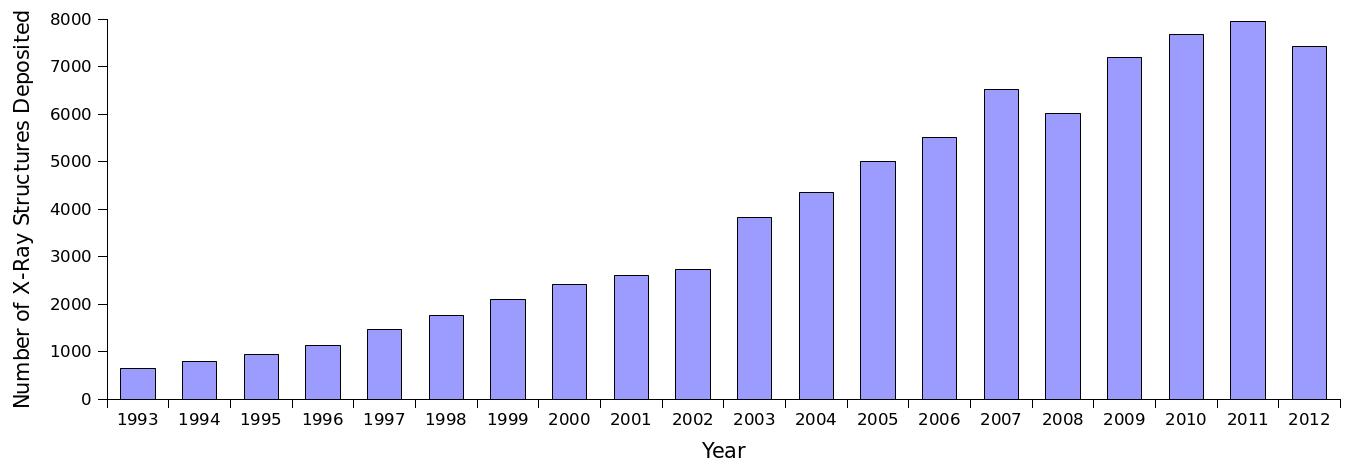
\includegraphics[width=\textwidth]{figures/pdb_deposit_rate.png}
\caption{The rate at which new structures is deposited into the PDB over the last two decades.
Due to a variety of improvements in the field of crystallography this rate has been steadily increasing.}
\label{figure:pdb_growth}
\end{center}
\end{figure}

% expected future growth of pdb
For example a recent increase in the field of crystallography, is ``crystal-less'' crystallography in which small molecules are bound by a porous scaffold matrix.
The regular structure of the matrix imparts a regular packing arrangement, necessary for interpreting diffraction patterns, onto the arrangement of small molecules.
This has the potential to address one of the largest difficulties in obtaining quality structural data for proteins, which is that it is very difficult to purify and crystallize certain proteins \cite{inokuma2013x}.

% unsorted
The number of target molecules of the set of all drugs currently available on the market consists of only about 500 proteins.
The bottleneck in introduction of new chemical entities is not virtual screening, but rather optimizing these hits into higher affinity leads and eventually balancing the requirements across all characteristics to produce a new drug \cite{bleicher2003hit}.

% unsorted
Of the total proteome only ~30,000 are regulated by small molecule binding, making them reasonable targets of drug action.
A large number of these possible drug targets are not implicated in any disease, due to this and a number of other factors, estimates of the total number of these proteins which are possible drug targets is much lower.
Frequently cited numbers for the number of possible drug targets in humans are six-hundred to fifteen-hundred, still significantly higher than the total number of targets which are exploited by current drugs.
The different families of cellular proteins are not equally likely to be targets of drugs.
As of {\the\year} 47\% of current drug targets are enzymes, followed by 30\% being GPCR's \cite{hopkins2002druggable}.

% drug-likeness
The consists of a number of characteristics which are generally true of drug like molecules:
\begin{enumerate}
\item Five or fewer hydrogen bond donors,
\item 500 Da or less total molecular mass
\item high liphophilicity
\item sum of nitrogen and oxygen atoms is not greater than 10 \cite{rule_of_five}
\end{enumerate}

% unedited
Through understanding the protein-ligand conformation and specific contacts they were able to modify a known substrate 
There is an advantage to flexible substrates, which is that they can flex in order to create better contacts with the protein structure increasing binding affinity.
This is especially important as the location of heavy atoms in the target protein is frequently only known to an accuracy of ~0.4 angstroms.
Further specific knowledge of the binding geometry between the initial lead compound and the target makes it possible to computationally screen possible chemical group substituents, to maximize binding affinity, increase solubility or bioavailability.
One of the earliest examples of the successful application of structure based drug design is the carbonic anhydrase inhibitor dorzolamide, in which most of these ideas were applied to find a drug with very high binding affinity \cite{greer1994application}.

% limitations
Despite advantages in speed and cost due to limitations in accuracy computational screening has struggled to produce the same results as empirical screening.
However, more recently virtual screening has succeeded in producing hit rates greater than those from empirical screening techniques.
Virtual screening has been used to identified leads which were later developed into the human immunodeficiency virus (HIV) protease inhibitor Viracept, and the anti-influenza drug Relenza.
\begin{figure}[h]
    \centering
    \begin{subfigure}[b]{0.3\textwidth}
        \centering
        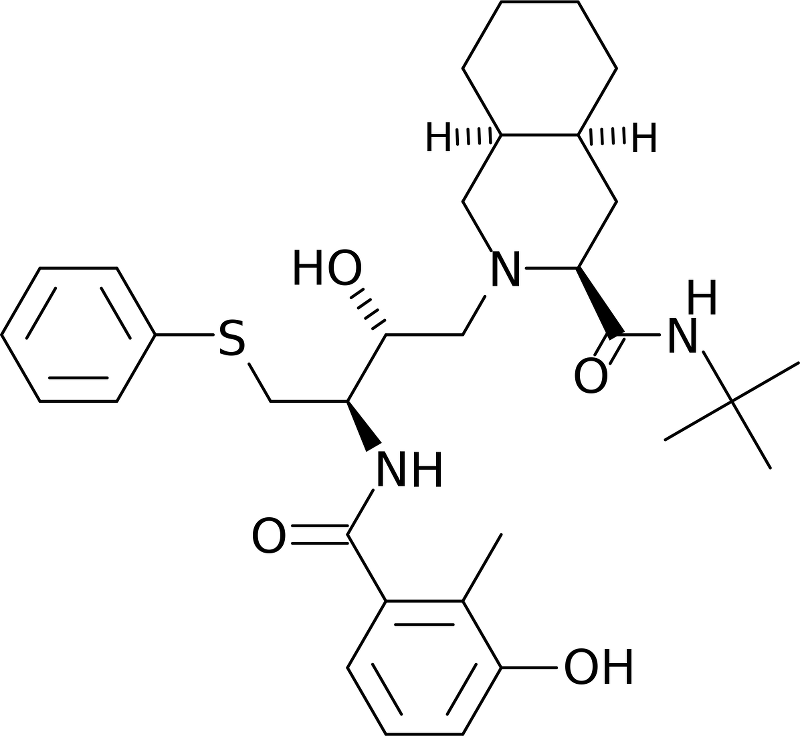
\includegraphics[width=\textwidth]{figures/nelfinavir_small.png}
        \label{fig:nelfinavir_chemical}
        \caption{}
    \end{subfigure}%
    \hspace{0.1\textwidth}
    \begin{subfigure}[b]{0.3\textwidth}
        \centering
        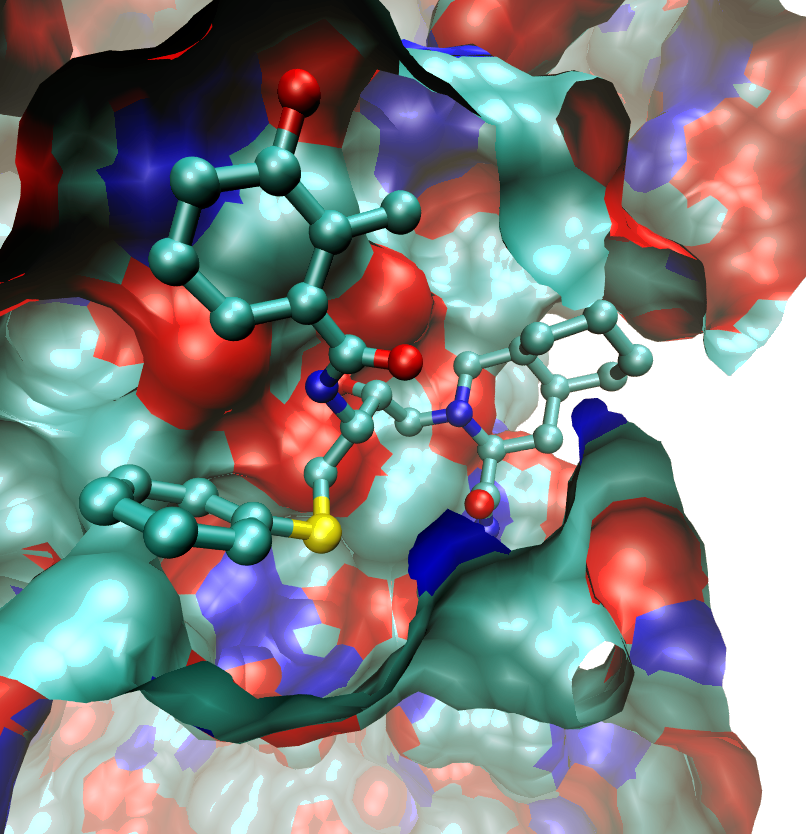
\includegraphics[width=\textwidth]{figures/complexed_nelfinavir_white.png}
        \label{fig:nelfinavir_docked}
        \caption{}
    \end{subfigure}
    \label{fig:nelfinavir}
    \caption{
The HIV protease inhibitor, nelfinavir, marketed under the name Viracept was originally identified using a computational docking screen.
It has a very high binding affinity for its target protein, 2 nM.
Here it is shown crystallized with multidrug variant (ACT) (V82T/I84V) of HIV-1 protease, PDBID 3EL5.
(b) generated with Visual Molecular Dynamics \protect\cite{humphrey1996vmd} and \protect\cite{povray}.
}
\end{figure}
A number of challenges which limit the utility of docking programs have been identified
\begin{enumerate}
\item The number of possible small molecules is essentially unbounded, however only a very small fraction of these ligands are potentially drug compounds. Limiting sampling to this subspace is a challenging problem.
\item The number of conformations of ligand molecules rises exponentially with the number of internal degrees of freedom of the ligand. Sampling the huge conformational space of the ligand becomes a computationally difficult problem on its own.
\item The difficulty of accurately assessing or comparing the energy of different protein-ligand complexes or conformations\cite{shoichet2004virtual}.
\end{enumerate}

% similarity between hits and leads
It has been found that introduced drugs are often very chemically similar the ``hit'' compounds from which they were derived \cite{proudfoot2002drugs}.
So in order to increase the diversity of drugs and find drugs which are able to treat new diseases, or diseases which have evolved resistance to current drugs it may be necessary to either increase the size of the screened database or increase the possible diversity which might be increase through the hit-to-lead step.

%\cite{kitchen2004docking}

\subsubsection{Hit-to-Lead Optimization}
\label{subsubsection:hit_to_lead}
Hit compounds generally have a binding affinity for the target protein on the order of micromolar binding.
The goals of hit-to-lead optimization are to further increase that affinity with the goal of eventually reaching binding affinities on the order of ~10 nanomolar or better, find other molecules with similar chemical characteristics to increase the size and diversity of the set of lead compounds, and screening hit compounds for any obvious issues.
At this stage for computational screening more accurate energy models are required than for the initial screen \cite{jorgensen2004many,gohlke2002approaches,jorgensen2009efficient}.
Depending on the type of ``hit'' compounds identified in the initial screen, hits are either combined through molecular-growing and evolution techniques, or similar structures to the hit compounds can be sampled either by exploring the local chemical space or ``mutation'' of substituents.
In either case, the potential lead compound is docked or grown in the known binding site.
A scoring function which is hopefully well correlated with the binding energy is then used to rank these possible compounds.
Interestingly it is not necessarily the case that the scoring function is anchored in a physical force field, it is possible to use statistical or artificial intelligence approaches with success, so long as they are able to successfully solve the classification problem of distinguishing strong binders from weak binders.
Docking as a means of converting hit compounds to lead compounds is very similar to docking as a means of hit generation, however in this case the small molecule library is much smaller and is generated to cover chemical space surrounding hit compounds.
Additionally whereas for initial hit generation a coarse grained energy function might have been sufficient to differentiate ligands which bind strongly from those which do not bind at all, to convert these ``hits'' to lead compounds it is necessary to use a more sensitive, and necessarily slower, energy model to accurately rank the binding affinity of different small molecules \cite{jorgensen2004many,gohlke2002approaches}.
These energy models will be discussed briefly in \ref{subsection:energy_functions}.

A popular program for building, or mutating lead compounds is Biochemical and Organic Model Builder (BOMB) \cite{barreiro2007docking}.
BOMB can operated as either a hit identification program or as a hit to lead optimization method.
Working to identify new compounds BOMB starts with a number of different small ``core'' scaffolds and attempts to increase binding affinity by adding or replace substituents with favorable interactions while avoiding steric clashes.
BOMB has been successfully used to evolve a hit compound which showed no inhibition of HIV reverse transcriptase into a potent non-nucleoside RT inhibitor with nanomolar level binding \cite{barreiro2007docking}.

Whereas previously, lead compounds were evaluated almost exclusively on binding affinity to the target protein, more recently more weight is being placed on identifying hit compounds which satisfy other characterisitcs besides binding affinity \cite{bleicher2003hit}.
It is important to begin to consider other characterisitcs of the potential drugs earlier in the pre-clinical process, because later it is difficult to make changes which affect characterisitcs such as solubility without significantly altering the binding affinity of an already highly modified hit compound.
As ``lead'' compounds are rarely very chemically distinct from the hits from which they were derived, and increasing binding affinity is actually sometimes an easier problem than addressing some of the other characteristics in the ``rule of five'' it is reasonable to begin by first trying to optimize hit compounds to satisfy some other criteria and postpone maximizing binding affinity \cite{proudfoot2002drugs}.

\subsubsection{Lead Optimization}
\label{subsubsection:lead_optimization}
In lead optimization the compounds which have been identified by the earlier steps in the process are optimized to drug molecules.
The largest differentiating factor between hit-to-lead optimization and lead optimization is the plausibility of the compound to act as a successful drug molecule.
The goals of lead optimization overlap heavily with those of the hit-to-lead stage.
Although this can include increasing binding affinity to the target even further, usually the focus is on other characteristics including selectivity, ease of synthesis, pharmacokinetic properties and intellectual property concerns \cite{keserHu2006hit}.
Computational modelling can help not only identify hit compounds, and convert those initial hits into leads, but also to help estimate absorption, distribution, metabolism, elimination, toxicology, sometimes referred to as the ADME characteristics \cite{kerns2008drug}.

Computational models for ADME characteristics ususally use regression equations or neural networks to predict these characteristics \cite{jorgensen2004many}.

Up to one half of all drugs which do not survive clinical trials, fail to do so because of lack of efficacy, which is influenced both by binding, but also by the absorption characteristics of the molecule.
The number of drugs which fail to make it through clinical trials due to toxcicity is similarly high, about 40\% \cite{li2001screening}.
Advancing a potential drug to clinical trials represents a very large financial investment, and effective computational screens of lead molecules at this point in the process can reduce the rate of failure in clinical trials, thereby having a very large impact on the final costs of new drugs brought to market.
